\documentclass[a4paper,10pt]{article}

\usepackage[utf8]{inputenc}
\usepackage[T1]{fontenc}
\usepackage[danish]{babel}

\usepackage{color}
\usepackage{float}
\usepackage{fancyvrb}

\usepackage{amssymb}
\usepackage{amsmath}
\usepackage{listings}
\usepackage{comment}
\usepackage{hyperref}
\usepackage{bookmark}
\usepackage{mathtools}

\usepackage{graphicx}
\usepackage[]{algorithm2e}
\DeclareGraphicsExtensions{.png}
\DeclarePairedDelimiter\floor{\lfloor}{\rfloor}

\definecolor{dkgreen}{rgb}{0,0.45,0}
\definecolor{gray}{rgb}{0.5,0.5,0.5}
\definecolor{mauve}{rgb}{0.30,0,0.30}
\definecolor{blue}{rgb}{0, 0, 0.45}
\definecolor{red}{rgb}{0.45, 0, 0}

% Default settings for code listings
% Default settings for code listings
\lstset{frame=tb,
  language=Java,
  aboveskip=3mm,
  belowskip=3mm,
  showstringspaces=false,
  columns=flexible,
  basicstyle={\small\ttfamily},
  numbers=left,
  numberstyle=\footnotesize,
  keywordstyle=\color{dkgreen}\bfseries,
  commentstyle=\color{dkgreen},
  stringstyle=\color{mauve},
  frame=single,
  breaklines=true,
  breakatwhitespace=false
  tabsize=1
}

%indsætjeres navn herunder.
\title{Introduction to Programming - Re-exam Project (Part II)\\\rule{10cm}{0.5mm}}
\author{Simon Dradrach Jørgensen 
\\Supervisor: Jan Baumbach\\ DM550 - Re-Exam\\\rule{5.5cm}{0.5mm}\\}
\date{\today}

\begin{document}

\maketitle

\vfill

\tableofcontents
%laver forside og indholsfortegnelse

\newpage
\section{Specification} 
%forklar hvad programmet skal gøre
The given task is to print an un-solved \textit{sudoku puzzle} to the user, which they're supposed to solve. This means an implementation of a \textit{GUI} is required, to show the output to the user, involving buttons to call functions that can load and save the file, (as long as it's a \textit{Sudoku puzzle layout}).

\textit{Sudoku puzzles} are a kind of crossword puzzles with numbers where the following two conditions have to be met: \cite{1}

\subsection{Condition 1} 
In each row or column, the nine numbers have to be from the \textit{set [1,2,3,4,5,6,7,8,9]} and they must all be different.

\subsection{Condition 2} 
For each of the nine non-overlapping 3x3 blocks, the nine numbers have to be from the \textit{set [1,2,3,4,5,6,7,8,9]} and they must all be different.

\section{Design}
%hvordan projektet blev planlagt, hvilke tanker gik ind i hvordan problemet skulle løses
The goal of the program, is to construct a \textit{user interface}, using the \textit{swing library} which is a part of the default \textit{java} library. Therenext, the user should be able to edit the "empty slots" with integers, to try to solve the \textit{sudoku puzzle}, and lastly the program needs to check, if the user is correct in their inputs.

A way to load any un-solved \textit{sudoku puzzle} is a requirement, since re-using the same layout over and over again is no challenge, thus a way to load a \textit{sudoku-template.txt} file can be implemented, and obviously a way to save that file when the user have completed the \textit{sudoku puzzle}. 

To make sure that the program can check up on users inputs, being either correct or wrong, therefore a way to check if there's any conflicting inputs with the already plotted integers are required, and also a way to forbid anything else than integers. To make sure that user understands when and where they made a mistake, a color can be used to show what's right and what's wrong, also where exactly in the \textit{sudoku puzzle}.

\newpage

\section{Implementation}
%hvordan skrev du programmet
%forklar hvordan delene af dit program virker
For the following task, a \textit{Field} class is required, creating two \textit{arrays}, each with the same constant, which are then multiplied to forge the \textit{sudoku table}, which is used for inserting the integers.

A numerous boolean functions were required, to make sure that the program could check where the inputs would be located. Since there's a single \textit{array}, formed by two other \textit{arrays}, these check functions are:

\begin{equation}
    f(y,v)=\forall x \in \ \mathbb{Z} \ \cap \ ]0:9] : data_{(x,y)} \ne v
\end{equation}

This function checks for all elements in a given row, and returns false, if the inserted integer is a duplicate of another integer already in the \textit{array}. Same goes for checking columns, but with [i][j] being swapped.

\begin{equation*}
    f(x, y, v) = \forall x' \in \ \mathbb{Z} \ \cap \ ]0:3],\forall y' \in \ \mathbb{Z} \ \cap \ ]0:3] : data_{(\floor*{\frac{x}{\sqrt{9}}}*3+x' , \floor*{\frac{y}{\sqrt{9}}}*3+y')} \ne v
\end{equation*}

Where \textit{v} is defined as the \textit{value}. In this function, the program checks what box one is currently occupying in.

\begin{lstlisting}[language=java]
public boolean tryValue(int val, int i, int j) {
        if (!checkRow(val, i) || !checkCol(val, j) || !checkBox(val, i, j)) {
            return false;
        }

        this.model[i][j] = val;
        return true;
    
    }
\end{lstlisting}

These functions returns false if the value cannot be placed in either the row, or the column.

\begin{lstlisting}[language=java]
public boolean isEmpty(int i, int j) {
        return model[i][j] == 0;
\end{lstlisting}

Is a function that checks for an empty space in the array.

\newpage

\subsection{Graphical User Interface}

The way the user inserts integers, works best by allowing them to write the given integer, in the cells. These cells however, needs to be changeable inside the \textit{UI} itself, requiring the use of the \textit{JTextField} class.However, the user needs a way to tell the program that they are done inserting integers, this was implemented via a \textit{JButton}. For the \textit{JButton} to actively change the \textit{JTextField}, a \textit{check} function was implemented, this function does the following:

\begin{itemize}
\item Warn the user if the integer conversion from the given string, failed.

\item Tells the user which variables are constant/fixed, and will redo any changes done to these cells

\item Tells the users whether or not an integer failed the \textit{sudoku check}, with a color scheme. \textcolor{blue}{\textbf{Blue}} if succeeded, and \textcolor{red}{\textbf{Red}} if failed.

\item Finally, it inherits the files way of telling, that the variable of a cell is unknown. This means that all \textbf{0}'s will be replaced, with \textbf{X}'s
\end{itemize}

To \textit{load} the wanted file, the \textit{load} function, incapable of setting the size of the \textit{sudoku table}, resets all the text fields, and the \textit{sudoku field}. The function will load all the integers from the \textit{sudoku} file, with the \textit{sudokus} in-built \textit{fromFile} function, where it will let the \textit{check} function replace all \textbf{0}'s with \textbf{X}'s as per fitting the \textit{sudoku} file \textit{scheme}.

The \textit{save} function is a bit more simple, it \textit{prints} the \textit{sudoku} file, and replaces all the "special character", e.g., $\{ + , - , | \}$ from the \textit{Field} class. The \textit{save} function however, does not need to replace all \textbf{0}'s with \textbf{X}'s, since there won't be any when the \textit{save} function is available to the user, given that they'd only be able to save when the \textit{sudoku} have been completed.

\section{Testing}

\begin{comment}
I testing skal i forklare jeres tests osv. udover det kan i have et billede med
som i kan tilføje ved at kopiere includegraphics som herunder.

\begin{figure}[H]\center
\includegraphics[scale=1]{billede.png}
\caption{}
\end{figure}

udskift billede.png med jeres billede fil som skal ligge i samme mappe som .tex
i kan ændre på scale for at ændre pÃ¥ billede størrelse i pdfen.
\end{comment}

To test the \textit{sudoku puzzle}, a solver was created to test if the program would only spit out the correct result when checking, e.g.,

\begin{lstlisting}[language=java]
Field field = new Field();
        field.fromFile(args[0]);
        try {
            solve(field, 0);
        } catch (SolvedException e) {
            System.out.println(field);
        }

public static void solve(Field f, int i) throws SolvedException {
        if (i >= Field.SIZE * Field.SIZE) {
            throw new SolvedException();
        }

        if (!f.isEmpty(i % Field.SIZE, i / Field.SIZE)) {
            solve(f, i + 1);
            return;
        }

        for (int x = 1; x <= Field.SIZE; ++x) {
            if (f.tryValue(x, i % Field.SIZE, i / Field.SIZE)) {
                solve(f, i + 1);
            }

        }
        f.clear(i % Field.SIZE, i / Field.SIZE);
    }
\end{lstlisting}

Given the program one of the \textit{test.sudoku.txt} files, it was possible to see if the solver could find an answer, and if the program could distinguish between a right and wrong input from the user. With this information, one could see the finished result, e.g.,

\begin{figure}[htp]\center
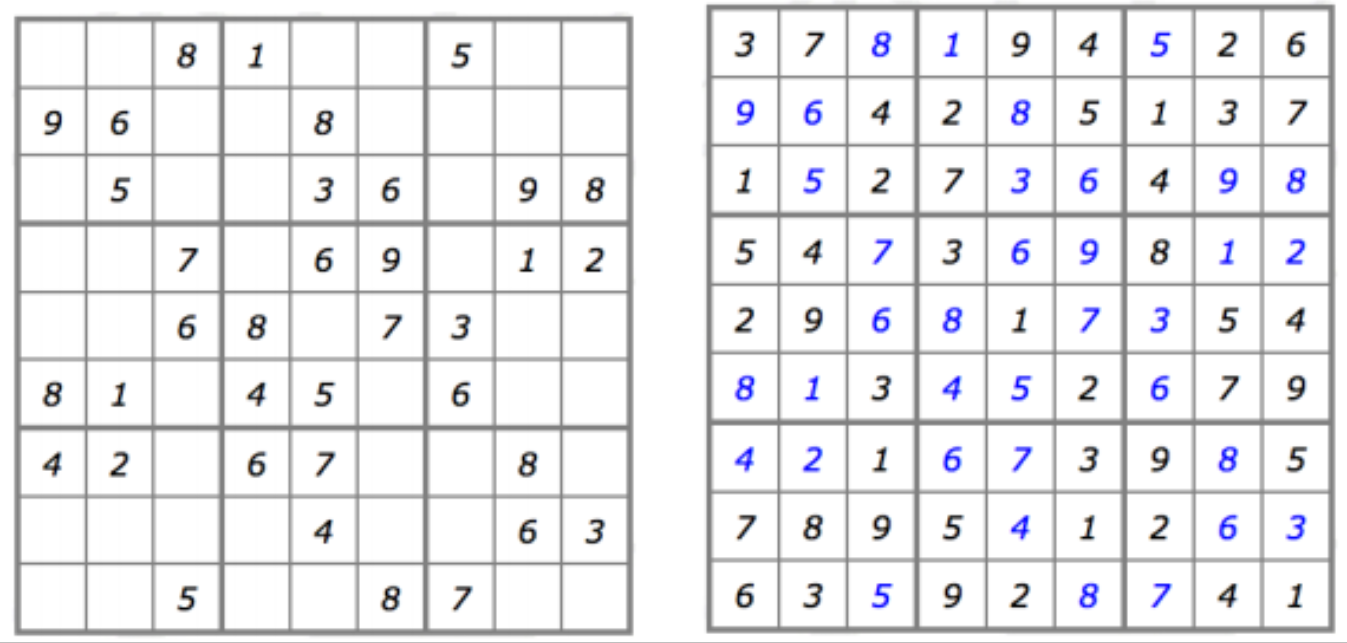
\includegraphics[scale=0.2]{sudoku.png}
\caption{Sudoku}
\end{figure}

One could then plot those integers given and see if the program accepted that as an answer. If it did, it'd prove to be correct.

This proved useful in the early stages of the program, due to the fact, that the user would get "false" everytime they'd click the \textit{check button}, even if there were no integer with \textit{n}-value in either \textit{row} 'nor \textit{column}. It was then easy to find the mistake and fix it.

\section{Conclusion} 
%hvad kom i frem til, gik noget galt? kunne noget gøres bedre?
With the useage of the \textit{swing} library, one can create a well-functioning \textit{GUI} for a \textit{sudoku puzzle}. It could however easily have been improved, by sepparating the 9 boxes in the \textit{sudoku table} by a grid of some type, to make it more clear that within those boxes, duplicates are not allowed. This could however been done, by using a \textit{class} that extends the \textit{swing} layout manager interface.

\newpage

\section{Appendix (source code)}
%lstinputlisting tilføjer jeres sourcecode, jeres python fil skal bare ligge i samme mappe som .tex filen husk at fjerne %

%\textbf{Sierpinski triangle program}
%\lstinputlisting[language=python]{sierpinski.py}
%\textbf{Binary tree program}
%\lstinputlisting[language=python]{binary.py}
\subsection{Field}
\begin{lstlisting}[language=java]
/**
 *
 * @author r41
 */
import java.io.*;
import java.util.*;

/**
 * Abstract Data Type for Sudoku playing field
 */
public class Field {

    public static final int SIZE = 9;

    public int model[][];

    public Field() {
//        make new array of size SIZExSIZE
        this.model = new int[SIZE][SIZE];
    }

    public void fromFile(String fileName) {
        try {
            Scanner sc = new Scanner(new File(fileName));
            fromScanner(sc, 0, 0);
        } catch (FileNotFoundException e) {
            // :-(
        }
    }

    private void fromScanner(Scanner sc, int i, int j) {
        if (i >= SIZE) {
            // all rows done!
        } else if (j >= SIZE) {
            // this row done - go to next!
            fromScanner(sc, i + 1, 0);
        } else {
            try {
                int val = Integer.parseInt(sc.next());
                this.model[i][j] = val;
            } catch (NumberFormatException e) {
                // skip this cell
            }
            fromScanner(sc, i, j + 1);
        }
    }

    @Override
    public String toString() {
        StringBuilder res = new StringBuilder();
        for (int i = 0; i < SIZE; i++) {
            if (i % 3 == 0) {
                res.append("+-------+-------+-------+\n");
            }
            for (int j = 0; j < SIZE; j++) {
                if (j % 3 == 0) {
                    res.append("| ");
                }
                int val = this.model[i][j];
                res.append(val + " ");
            }
            res.append("|\n");
        }
        res.append("+-------+-------+-------+");
        return res.toString();
    }

    /**
     * returns false if the value val cannot be placed at row i and column j.
     * returns true and sets the cell to val otherwise.
     */
    public boolean tryValue(int val, int i, int j) {
        if (!checkRow(val, i) || !checkCol(val, j) || !checkBox(val, i, j)) {
            return false;
        }

        this.model[i][j] = val;
        return true;

    }

    /**
     * checks if the cell at row i and column j is empty, i.e., whether it
     * contains 0
     */
    public boolean isEmpty(int i, int j) {
        return model[i][j] == 0;
        //if value is 0, it'll return true
    }

    /**
     * sets the cell at row i and column j to be empty, i.e., to be 0
     */
    public void clear(int i, int j) {
        model[i][j] = 0;
    }

    /**
     * checks if val is an acceptable value for the row i
     */
    private boolean checkRow(int val, int i) {
        for (int rowN = 0; rowN < SIZE; rowN++) {
            if (val == model[i][rowN]) {
                return false;
            }
        }
        return true;
    }

    /**
     * checks if val is an acceptable value for the column j
     */
    private boolean checkCol(int val, int j) {
        for (int columnN = 0; columnN < SIZE; columnN++) {
            if (val == model[columnN][j]) {
                return false;
            }
        }
        return true;
    }

    /**
     * checks if val is an acceptable value for the box around the cell at row i
     * and column j
     */
    private boolean checkBox(int val, int i, int j) {
        final int s = (int) Math.sqrt(SIZE);
        /**
         * square root of the size of the two arrays, resulting in 9 which is
         * the amount of boxes a typical Sudoku have
         */
        final int x = i / s * s, y = j / s * s;
        //checks what box one is occupying in
        for (int columnN = 0; columnN < s; ++columnN) {
            for (int rowN = 0; rowN < s; ++rowN) {
                if (model[columnN + x][rowN + y] == val) {
                    return false;
                }
            }
        }
        return true;
    }
}
\end{lstlisting}
\newpage
\subsection{Main}
\begin{lstlisting}[language=java]
import javax.swing.JFrame;

/**
 *
 * @author r41
 */
public class Main {

    public static void main(String[] args) {
        GUI window = new GUI();
        window.setDefaultCloseOperation(JFrame.EXIT_ON_CLOSE);
        window.setVisible(true);

        Field field = new Field();
        field.fromFile(args[0]);
        try {
            solve(field, 0);
        } catch (SolvedException e) {
            System.out.println(field);
        }

    }

    public static void solve(Field f, int i) throws SolvedException {
        if (i >= Field.SIZE * Field.SIZE) {
            throw new SolvedException();
        }

        if (!f.isEmpty(i % Field.SIZE, i / Field.SIZE)) {
            solve(f, i + 1);
            return;
        }

        for (int x = 1; x <= Field.SIZE; ++x) {
            if (f.tryValue(x, i % Field.SIZE, i / Field.SIZE)) {
                solve(f, i + 1);
            }

        }
        f.clear(i % Field.SIZE, i / Field.SIZE);
    }

}
\end{lstlisting}
\newpage
\subsection{Gui}
\begin{lstlisting}[language=java]
import java.awt.BorderLayout;
import java.awt.Color;
import java.awt.Dimension;
import java.awt.Font;
import java.awt.GridLayout;
import java.awt.event.ActionEvent;
import java.awt.event.ActionListener;
import java.awt.event.MouseAdapter;
import java.awt.event.MouseEvent;
import java.io.FileWriter;
import java.io.IOException;
import java.util.logging.Level;
import java.util.logging.Logger;
import javax.swing.*;

/**
 *
 * @author r41
 */
public class GUI extends JFrame {

    public Field field;
    public JButton checkbutton = new JButton("Check");
    public JPanel area = new JPanel();
    public boolean[][] fixed = new boolean[Field.SIZE][Field.SIZE];
    //checker for true or false in the 9x9 arrays

    public JMenu menu() {
        JMenu file = new JMenu("File");
        String names[] = {"open file", "save file"};

        MouseAdapter actions[] = {
            new MouseAdapter() { // Open file action
                @Override
                public void mousePressed(MouseEvent e) {
                    JFileChooser fileChooser = new JFileChooser();
                    if (fileChooser.showOpenDialog(null)
                            == JFileChooser.APPROVE_OPTION) {
                        load(fileChooser.getSelectedFile().getPath());
                    }
                }
            },
            new MouseAdapter() { // Save file action 
                @Override
                public void mousePressed(MouseEvent e) {

                    for (int j = 0; j < Field.SIZE; j++) {
                        for (int i = 0; i < Field.SIZE; i++) {
                            if (field.isEmpty(j, i)) {
                                JOptionPane.showMessageDialog(null, "Sudoku needs to be finished, before saving is an option.");
                                return;
                            }
                        }
                    }

                    JFileChooser fileChooser = new JFileChooser();
                    fileChooser.setApproveButtonText("Save");
                    if (fileChooser.showOpenDialog(null)
                            == JFileChooser.APPROVE_OPTION) {
                        save(fileChooser.getSelectedFile().getPath());
                    }
                }
            }
        };
        for (int i = 0; i < names.length; ++i) {
            JMenuItem j = new JMenuItem(names[i]);
            j.addMouseListener(actions[i]);
            file.add(j);
        }
        return file;

    }

    private void load(String path) {
        field = new Field();
        field.fromFile(path);
        for (int j = 0; j < Field.SIZE; ++j) {
            for (int i = 0; i < Field.SIZE; ++i) {
                JTextField txt = (JTextField) area.getComponent(i + j * Field.SIZE);
                String str = Integer.toString(field.model[j][i]).trim();    
                txt.setText(str.equals("0") ? "X" : str);
                txt.setHorizontalAlignment(JTextField.CENTER);
                txt.setBackground(Color.WHITE);
                fixed[j][i] = !field.isEmpty(j, i);
            }
        }

    }

    private void save(String path) {

        final String space = " ";
        try (FileWriter sv = new FileWriter(path, true)) {
            sv.write(field.toString().replace("+", space).replace("-", space).replace("|", space).replace("0", "X"));
        } catch (IOException ex) {
            Logger.getLogger(GUI.class.getName()).log(Level.SEVERE, null, ex);
        }
    }

    public GUI(String path) {
        this();
        this.load(path);
    }

    public GUI() {
        this.setLayout(new BorderLayout());
        this.add(area, BorderLayout.CENTER);
        this.add(checkbutton, BorderLayout.SOUTH);
        checkbutton.addActionListener(new ActionListener() {
            @Override
            public void actionPerformed(ActionEvent e) {
                for (int j = 0; j < Field.SIZE; ++j) {
                    for (int i = 0; i < Field.SIZE; ++i) {
                        JTextField txt = (JTextField) area.getComponent(i + j * Field.SIZE);
                        if (fixed[j][i]) {
                            txt.setText(Integer.toString(field.model[j][i]));
                        } else {
                            if (txt.getText().trim().toLowerCase().equals("x")) {
                                continue;
                            }
                            try {
                                int r = Integer.parseInt(txt.getText());
                                Color back = field.tryValue(r, j, i) ? Color.BLUE : Color.RED;
                                txt.setBackground(back);
                            } catch (NumberFormatException ne) {
                                txt.setText("X");
                                JOptionPane.showMessageDialog(null, "Only accepts integers.");
                                return;
                            }
                        }

                    }
                }
            }
        });
        final int dim = 50;
        checkbutton.setPreferredSize(new Dimension(dim, dim));
        JMenuBar bar = new JMenuBar();
        bar.add(this.menu());
        this.setJMenuBar(bar);
        final int gap = 10;
        area.setLayout(new GridLayout(Field.SIZE, Field.SIZE, gap, gap));
        area.setBackground(Color.BLACK);
        for (int i = 0; i < Field.SIZE * Field.SIZE; ++i) {
            final int size = 25;
            final int fsize = 25;
            JTextField txt = new JTextField();
            txt.setPreferredSize(new Dimension(size, size));
            txt.setFont(new Font(txt.getFont().getName(), Font.PLAIN, fsize));
            txt.setBorder(javax.swing.BorderFactory.createEmptyBorder());
            area.add(txt);
        }
        this.pack();
    }
}
\end{lstlisting}

\subsection{SolvedExceotion}
\begin{lstlisting}[language=java]
/**
 *
 * @author r41
 */
public class SolvedException extends Exception {
    
}
\end{lstlisting}

\begin{comment}
Hvis Fern Time er lavet tilføjes det her og begin og end comment skal fjernes. 
\textbf{Fern program}
\lstinputlisting[language=python]{fern.py}

\end{comment}

\medskip
 
\begin{thebibliography}{9}
\bibitem{1}
Jan Baumbach 

University of Southern Denmark 

\url{http://www.imada.sdu.dk/~jbaumbac/download/teaching/ws16-17/DM550/project/re-exam_introduction_to_programming_java_project.pdf}
 
\end{thebibliography}


\end{document}